%%!TEX TS-program = latex
\documentclass[12pt,letterpaper]{article}
\usepackage{epsfig}                 
\usepackage[authoryear]{natbib}
\usepackage{graphicx}
\usepackage{amsmath}
\usepackage{psfrag}
\usepackage{mathabx}
\renewcommand{\baselinestretch}{1.6}
\large
\pagenumbering{arabic}
\usepackage[usenames,dvipsnames]{color}
\usepackage{fullpage}
\bibliographystyle{genetics}
\usepackage{multirow}
\newcommand{\ye}{\hat{y}}
\newcommand{\xe}{\hat{x}}
\usepackage{color}
\usepackage[normalem]{ulem}  
	\newcommand{\gc}[1]{{ \color{red} #1}}
	\newcommand{\yb}[1]{{ \color{blue} #1}}




%Why do animals allow male control of female meiosis?
%Why does female meiosis allow the opportunity for exploitation by selfish sperm?
%sperm and egg genomes both favour the peaceful resolution of female meiotic drive
%strange bed fellows

%\title{Why does female meiosis allow the opportunity for exploitation by selfish sperm? BETTER TITLE?}
\title{
%Co-operation between the sexes trumps selfish control of female  meiotic drive. 
%Or 
Sperm do not evolve to collaborate in female meiotic drive. 
%Or Why does female meiosis allow the opportunity for exploitation by selfish sperm? 
}

\author{Yaniv Brandvain \\ email: ybrandvain@gmail.com  \and Graham Coop \\ email: gmcoop@ucdavis.edu }

\usepackage{fancyhdr}
\pagestyle{fancy}
\lhead{}
\rhead{}
\renewcommand{\headrulewidth}{0.0pt}
\rfoot{}
\cfoot{\thepage}
\date{}
\bibliographystyle{plain}
\begin{document}
\maketitle
\begin{center}
Center for Population Biology \& Department of Evolution and Ecology \\ University of California - Davis \\ Davis, CA, 95616
\end{center}

%FIgures 
{\bf Abstract:}
Because only one of four products of female meiosis is transmitted to offspring, oogenesis is particularly
	 susceptible to genomic conflicts arising when alleles gains in frequency at a cost to organismal fitness. 
In fact, many facets of oogenesis have been interpreted as mechanisms of protection against genomic outlaws. 
Why then is female meiosis often left uncompleted until after fertilization - 
	potentially providing an opportunity for sperm to meddle with its outcome and facilitate meiotic drive? 
The population genetic theory presented herein suggests that
	sperm nearly always evolve to increase the fairness of female meiosis when possible. 
These results are constant with current knowledge of sperm-dependent meiotic drivers, 
	and suggest that the requirement of fertilization for the completion of meiosis may represent 
	yet another mechanism of female meiosis designed to prevent meiotic drive.
\newpage

\section*{Introduction}
Despite the apparent unity of the organism, alleles can
gain an evolutionary advantage at a cost to  individual fitness
\citep{Burt2006}, often by exploiting meiosis and gametogenesis.
Because only one of the four products of female meiosis is transmitted to the egg, female meiosis is particularly vulnerable to such exploitation \citep{Sandler1957,Pardo-ManuelDeVillena2001a}. 
An allele that biases female meiosis in its favor (i.e. a meiotic driver), may increase in frequency even if this driver entails a pleiotropic fitness cost \citep{Prout1973}, generating a genetic conflict between the success of the driver and organismal fitness.
Meiotic drivers observed in both plants
\citep{Buckler1999,Fishman2005,Fishman2008}, and animals
\citep{Agulnik1990,Wu2005,Pardo-ManuelDeVillena2001c} highlight this
conflict -- the selfish benefits of drive and the associated
pleiotropic fitness costs sustain a balanced polymorphism
\citep{Prout1973}, 
and often generate ongoing evolutionary escalations of drive suppressors and enhancers \citep{Dawe1996,Fishman2008}. 
The threat of meiotic drive to organismal fitness is potentially so
severe that many basic properties of
meiosis and o\"{o}genesis, including the initial genome doubling in
meiosis I \citep{Haig1991}, arrested female meiosis
\citep{Mira1998}, centromere machinery \citep{Malik2002a,Malik2009,Malik2009}, and sex differences in the recombination rate \citep{Haig2010,Brandvain2012} 
have perhaps evolved to enforce fairness by disrupting meiotic drive \citep{Rice2013}.

It is therefore somewhat surprising that despite the intense evolutionary pressure on female meiosis to prevent meiotic drive, 
it is potentially open to sabotage by a virtual stranger -- a haploid sperm genome.
That is, in many animal species, female meiosis is completed only after fertilization \citep{Masui_book}, 
creating ample opportunity for interaction between the sperm and female meiotic machinery. 
Therefore, a `green-bearded' \citep{Gardner2010} sperm-acting allele that recognizes and facilitates the meiotic drive of a genetically equivalent allele in female meiosis %(a  heteromorphic dyad), 
     could presumably rapidly spread through a population. 
At first sight, female meiosis appears primed for exploitation by such selfish systems.  
Why then is the requirement of fertilization to complete female meiosis so ubiquitous? 

It is certainly not the case that animals are mechanistically incapable of circumventing this requirement.
The stage at which female meiosis requires fertilization varies widely across taxa, and in a few animals, 
	female meiosis is complete upon ovulation (that is, fertilization is not required for female meiosis \citep[see table 1 of ref 
][]{Masui_book}). 

It is also not the case that sperm is mechanistically incapable of influencing female meiosis.
In \emph{C. elegans}, premature deployment of the aster, a vital component of mitotic
machinery provided by the sperm, disrupts MII meiotic segregation
in the egg, leading to a triploid zygote \citep{McNally2012}. 
Thus, there is direct mechanistic evidence that sperm can influence female meiosis.
 Additionally, genetic evidence from the \emph{In} and \emph{Om}  drive systems in mice suggests that the 
 transmission of alternate alleles in heterozygous females can depend on sperm haplotype.  
 While ruling out the alternative hypothesis of early selection on zygotes \citep[pages
52-54][]{Burt2006} in these cases is challenging, it appears that the extent to which \emph{In} and \emph{Om} distort the second female meiotic division partially depends on the genotype of the fertilizing sperm \citep{Agulnik1993,Wu2005}.  
% Both of these female drive systems operate by distorting the second meiotic division, 
% and in both systems the outcome of female meiosis depends the genotype of the fertilizing sperm \citep{Agulnik1993,Wu2005}.  
%While such genetic evidence is suggestive, we note the difficulty in
%ruling out the alternative hypothesis of early selection on zygotes \citep[pages
%52-54][]{Burt2006}.


We develop population genetic models exploring the evolution of sperm influence on female meiotic drive, focussing on models in which `self-promoting' alleles in sperm facilitate drive of like genotypes during gametogenesis in heterozygous females.  
%In this article we explore through simple population genetic models the consequences of alleles that influence the outcome of female meiosis.
These models show that sperm modifiers of female meiotic drive are
unlikely to create a sustained conflict, and therefore 
female meiosis will have little incentive to evolve resistance to them.
In fact, the interests of sperm and egg  genomes' are often aligned, as both are invested in the fate of the resultant zygote (as was speculated for the \emph{In} locus \citep{Pomiankowski1993}).
Therefore, there is little selective benefit to females in preventing sperm to influence female meioses,
	indeed features of meiosis may evolve that facilitate the interaction of sperm with female meiosis. 

\section*{Results}

\subsection*{ Invasion of the population by a driving allele that promotes
itself.}
%%%%%%%%%%%%%%%%%%%%%%%%%
% PLEIOTROPY MODEL [self-promoting]
%%%%%%%%%%%%%%%%%%%%%%%%%

In the standard single-locus, biallelic model of female meiotic drive,
the driving allele is transmitted to the egg  in heterozygotes with
probability  $d > 1/2$, regardless of sperm genotype. To depict a case
of a self-promoting meiotic driver,  we modify this standard model such 
	that the driver is only effective when fertilized by a sperm carrying that allele (see Figure \ref{Eggsperm_2_allele_cartoon})
\footnote{the timing of fertilization relative to female meiosis places another constraint on $d$, for example, if fertilization (and therefore, sperm dependent drive) takes place at MII (as in mammals),
	female drive requires an uneven number of crossovers between the centromere and the drive locus, 
	so $d$ is bounded to be $<0.75$? \citep[see ][ for
        discussion]{Buckler1999}. }. %PUT THIS BACK IN
We then identify the conditions allowing for the spread of this self-promoting driver, 
	and evaluate whether a driver of this form could generate a sustained conflict favoring the evolution of suppressors. 

For comparative purposes, we present the standard drive model as Model 1 in the Appendix, 
%equations \ref{eqn.A1}-\ref{eqn.A3}, 
	and refer readers to the previous literature on this model \citep[e.g. ][]{Prout1973,Ubeda2004} for additional results. 
In this case, assuming the driving allele is deleterious in both sexes but fully recessive 
	(i.e. the fitness of drive homozygotes equals $w_{BB}=1-s$ and other genotypic fitnesses equal $w_{AA}=w_{AB}=1$), 
	it always invades because,  when rare, it occurs predominantly in heterozygotes and therefore drives without a fitness cost. 
However, when $s$ is large ($s>(2d-1)/(2)$) a driver cannot fix, and
will be maintained as a protected polymorphism \citep{Prout1973}. The
        parameter space where the allele can invade but not fix is shown in white
        in Figure \ref{Invasion_space}A, and where it can fix in the green
        and orange areasin Figure \ref{Invasion_space}B. When the allele is
        maintained as a polymorphism, it provides an opportunity for the evolution of
	drive suppressors, corresponding well to empirical examples of
        female meiotic drive \citep[reviewed in ][]{Burt2006}. 

In contrast to a traditional driver, which drives but pays effectively
	no fitness cost when rare, 
	a self-promoting driver specifically creates homozygote
        zygotes when it drives. %in heterozygotes. 
%, and therefore there is a drive-associated fitness cost even when rare. 
It must therefore overcome a drive-associated homozygous fitness cost simply to spread when rare. 
The conditions allowing the invasion of a self-promoting driver
 	are consequently far more restrictive than those for a standard meiotic driver.
When rare, a fully recessive, self-promoting driver can only invade when $s$ 
	%, the selection against the drive homozygote, 
	is less than $(2 d - 1)/(4 d)$. 
This analytical approximation, derived from Equation \eqref{deltadriver} assuming Hardy-Weinberg, 
	closely matches results obtained by exact numerical iteration (Figure \ref{Invasion_space}). 


When a self-promoting driver does spread, 
	it spends much time at low frequency, 
	because the paucity of complimentary sperm compromises its ability to drive. 
However, once relatively common, it  rapidly achieves fixation due to its
	positive frequency dependent behavior (Inset in Figure \ref{Invasion_space}).  
This lack of a balanced polymorphism %(Figure \ref{Invasion_space}) 
	precludes the evolution of an
	allele that suppresses this form of meiotic drive in females.

%I SUBSTANTIALLY REWROTE THIS
The positive frequency dependence of a self-promoting driver can
induce bistability in its spread.
%OLD GRAHAM WORDS
 %, i.e. there is a critical frequency
%above which it can spread quickly to fixation and below which it moves towards loss (an
%unstable equilibrium frequency). In 
%the appendix, we develop a simple
%approximation to this bistability. 
When $s$ is too large to allow a rare driver to increase in frequency, but small enough to allow a common driver to fix (the inequality in Equation \ref{ineqA}),
there is  an unstable equilibrium frequency, $f^*_{B\text{ recessive}}$  
	above which it can spread quickly to fixation and below which it moves towards loss 
	($f^*_{B\text{ recessive}}$ is approximated in Equation \ref{bistab_homozy_approx}.  
	We compare this approximation to the exact result in Figure \ref{Bistab_homozyg_cost_fig}).	
%OLD GRAHAM WORDS
%This bistability occurs in the region of parameter space in Figure
%\ref{Invasion_space}. In Supplementary Figure
%\ref{Bistab_homozyg_cost_fig} we further explore this bistability and
%show that the unstable equilibrium frequency is high across much of
%this parameter space, and so in practice the self promoting allele
%only invade in the orange space. (In the appendix we develop a simple
%approximation to the unstable equilibrium frequency
%\eqref{bistab_homozy_approx} that is also shown in  Supplementary Figure
%\ref{Bistab_homozyg_cost_fig}).
This unstable equilibrium frequency is high across much of
	parameter space, likely too high to be reached by drift, 
	and therefore  the fate of self-promoting drivers  will  likely be determined
	by the more restrictive invasion criteria rather than the fixation criteria. 


%OLD YANIV WORDS
% Compared to the invasion criteria, the parameter space
% allowing the fixation of the allele if it is above a cutoff frequency is much broader -- 
% 	a common, recessive, self-promoting driver fixes if
%         $s<(2d-1)/2$ approximately. 
% Therefore, when $(2 d - 1)/(4 d)<s<(2d-1)/(2)$, 
% 	a recessive, self-promoting driver will deterministically fix if drift, mutation, 
% 	or migration pressure bring its frequency above $(1-2d+4ds)/(2s(2d-1))$, 
% 	but it will be lost otherwise.
Inclusion of a heterozygous fitness cost (i.e. $w_{AB}=1-s_h$)
further constrains the evolution of a self-promoting driver. 
In fact, with any heterozygous fitness cost, a rare self-promoting
driver cannot spread deterministically. 
However, this case also displays bistability -- 
	mathematical approximation assuming Hardy-Weinberg reveal that 
	if $s < d - 1/2+s_h(3-2d)/2$, it will fix deterministically if its 
	frequency is greater than a threshold, $f_B^*$ [Equation \eqref{thresh2}. 
	See \yb{FIGURES SXX} for exact results].
%	because it pays the  heterozygous fitness cost but drives
 %      ineffectively (see Figure S\ref{bistable_additive})
%While a standard female driver invades from low frequency when the transmission advantage outweighs the fitness cost (XXX),
%	a rare self-promoter pays a fitness cost, but drives only weakly because complementary sperm are uncommon. 
%This frequency-independent fitness cost, and positive frequency dependent drive generates a bistable system. 
%Below a cutoff frequency the self-promoter driver deterministically decreases in frequency 
%	because it pays the  heterozygous fitness cost but drives
 %      ineffectively (see Figure S\ref{bistable_additive}). 
%Above this frequency, the allele increases deterministically because the commonness of complementary sperm 
%	make drive effective enough to overcome the associated fitness cost.
This bistability prevents self-promoting drivers from invading 	
	reasonably sized populations, and assures that, if they do invade, they will rapidly fix.
Our model therefore predicts that self-promoting drivers will not be
	observed as stable polymorphisms in natural populations. 

Although the allelic identity of sperm could plausibly influence the outcome of female meiosis, 
	limited gene expression in sperm \citep[e.g.][]{Joseph2004}
	suggest a model where sperm influence female meiosis via expression of the fertilizing male's
	diploid genotype (perhaps due to proteins and RNAs packaged into the sperm), rather than sperm haplotype.
This male-genotype dependent model requires one additional parameter, as we exchange $d$ in the sperm dependent case for $d_{het}$ and $d_{hom}$ which describe the transmission of the drive allele in a heterozygous female mating with males heterozygous and homozygous for the self-promoting drive allele, respectively.  
Here, a rare driver invades when $s$ is less than $(d_{het}-1/2)/d_{het}$, and usually fixes when it invades.
	% fixes when $s$ is less than $d_{hom} - 1/2$.
However, when the distorting effect of genotype displays strong dominance in its
	effect on female meiosis ($d_{het}$ is close to $d_{hom}$), 
	there is a a narrow sliver of parameter space sustains a polymorphism
	when the cost of the drive is recessive
	(see Figure S\ref{Effect_of_dominance}, \yb{and Equation \ref{polymale}}).  
%Presumably this zone of polymorphism comes about because positive frequency 
%	dependence diminishes with the dominance of the male effect driver. 
%As an analytical example, consider the case of male-genotype dependent deleterious recessive female driver (assuming, as above, $w_{BB}=1-s$, and $w_{AA}=w_{AB}=1$). 
%Here, a rare driver invades when $s$ is less than $(d_{het}-1/2)/d_{het}$, and fixes when $s$ is less than $d_{hom} - 1/2$.
%Intermediate values of $s$, which represent a small proportion of parameter space can maintain a polymorphism. 
While mathematically interesting, it does not seem particularly realistic to think that the
	effect of the drive allele would be dominant in its action through the
	male genotype, while the cost would be recessive. 
Therefore, although this model can sustain a polymorphism, 
	the lack of biological reality underlying the small portion of parameter values 
	required for this polymorphism make us doubt it general applicability. 
%Thus we regard this case as interesting but not very general.


Given the difficulty that self-promoting meiotic drivers have entering the population, the speed at
which they fix if they do, and the narrow parameter range permitting balanced polymorphisms at such loci,  
it seems very unlikely that such alleles could drive the evolution of female suppressors of sperm-enabled
female meiotic drive.

\begin{figure}
	\rotatebox{90}{
\includegraphics[width = 0.5
          \textwidth]{Figures/Sperm_egg_cartoon_paper_Fig1.eps}}
\caption{transmission probabilities for alleles through female
  meiosis depend on sperm genotype. 2 allele model}  
\label{Eggsperm_2_allele_cartoon}
\end{figure}


% (we note that the timing of fertilization relative to female meiosis places another constraint on $d$, for example, when drive takes place druing the second meitoic division
%	it requires an uneven number of crossovers between the centromere and the drive locus \citep[see ][ for discussion]{Buckler1999}). 

\begin{figure}
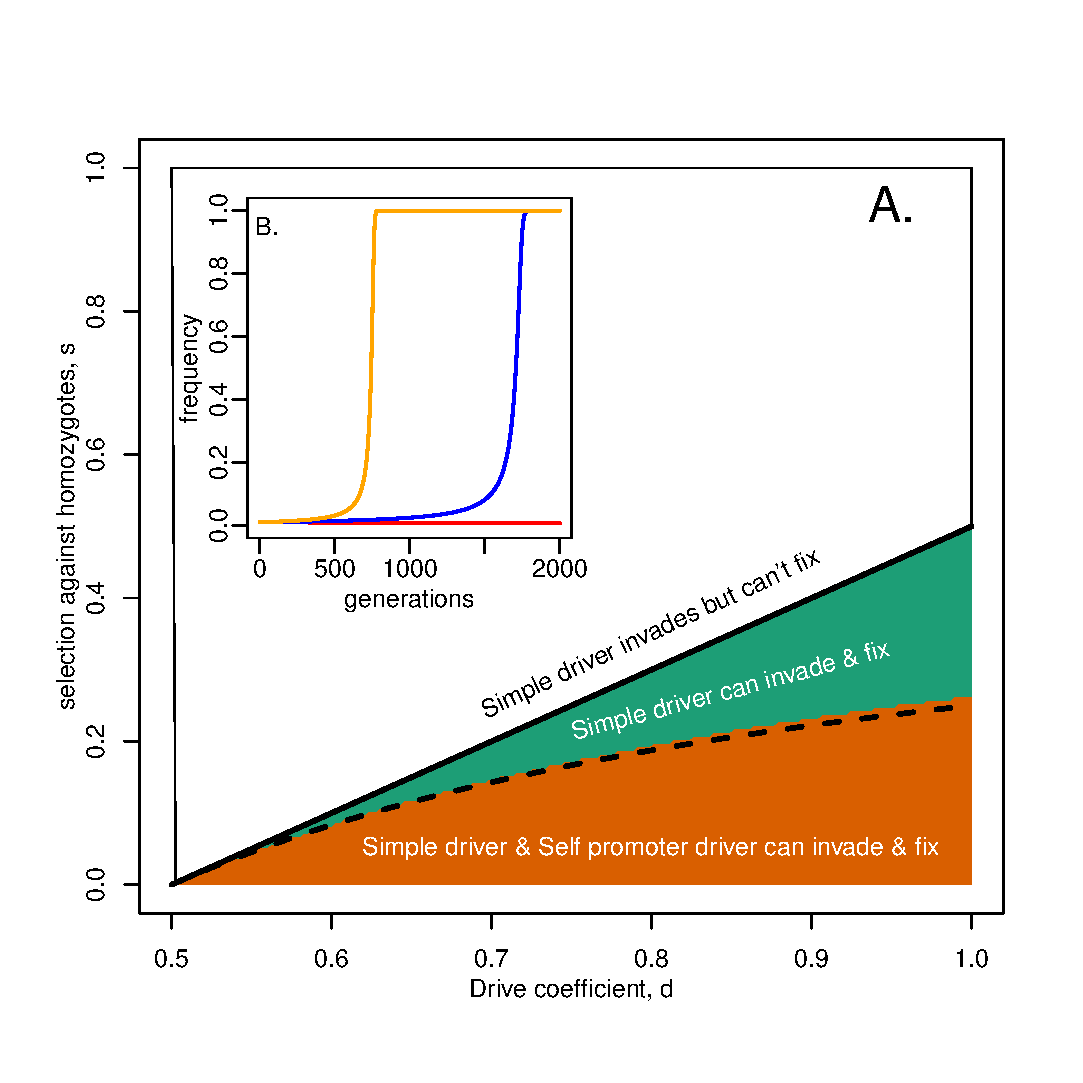
\includegraphics[width = 0.8 \textwidth]{Figures/invasion_space_recessive_driver.eps}
\caption{{\bf A.} Invasion analysis for a female meiotic drive allele with
  recessive costs (selection coefficient $s$). First consider a simple female meiotic
  drive system, where the allele is transmitted a fraction $d>1/2$ of
  meioses in female heterozygotes, inspective
  of the allele carried by the fertilizing sperm. 
Such an allele can invade the population over all of the parameter space, and will be maintained as a
  protected polymorphism in the white region, and can fix in the
  population in all of the parameter space colored green or orange. 
The solid back line marks the criteria for the allele to fix $s< (2d-1)/2$.
Now consider an allele that is fairly transmitted through
  female meiosis when fertilized by a sperm carrying a different
  allele, but at a fraction $d>1/2$ when a heterozygote egg is fertilized
  by a sperm carrying the allele (as depicted in Figure
  \ref{Eggsperm_2_allele_cartoon}). Such an allele can only invade in
  the region of parameter space colored orange, and it fixes over all
  of this parameter region. The approximate criteria for this allele
  to fix is given by the dashed line showing $s < (2d- 1)/(4d)$. 
 {\bf B.} In the inset we show trajectories of sperm-dependent female drive
 alleles that can invade the population, each allele has $s =0.1$ against the
 homozygotes and $d =0.6$, $0.7$, $0.8$ shown in yellow, blue, and red. 
 \gc{Likely make this Figure 1B.} } \label{Invasion_space}
\end{figure}


\subsection*{ sperm-egg haplotype balanced drive systems}

\begin{figure}
	\rotatebox{90}{\includegraphics[width = 0.8
          \textwidth]{Figures/Sperm_egg_cartoon_paper_Fig2.eps}}
\caption{Dynamics in 3 allele system
{\bf (A) } The sperm-dependent transmission probabilities of alleles through
female meiosis (female germ cells depicted as circles, sperm indicated by wiggly
tails). In each case the top and bottom entry in each cell give the
transmission probability of the left and right allele in the female
being transmitted to the egg. In the left panel we show the transmission probabilities for
  A, B, and B'. Where B' is a driver allele which is either promotes
  itself through through female meiosis when sperm (a B$^+$ allele,
  $d'>d$) or self-avoiding through the interaction of sperm with female meiosis (a B$^-$ allele,
$d'<d$). In the right panel we depict the transmission probabilities for
  A, B, and A$^-$ allele a non-driven allele that acts to reduce the
  effects of female drive through sperm.
{\bf (B)} Frequency trajectories in the three allele system. }
 \label{Eggsperm_3_allele_cartoon}
\end{figure}


% \begin{figure}
% 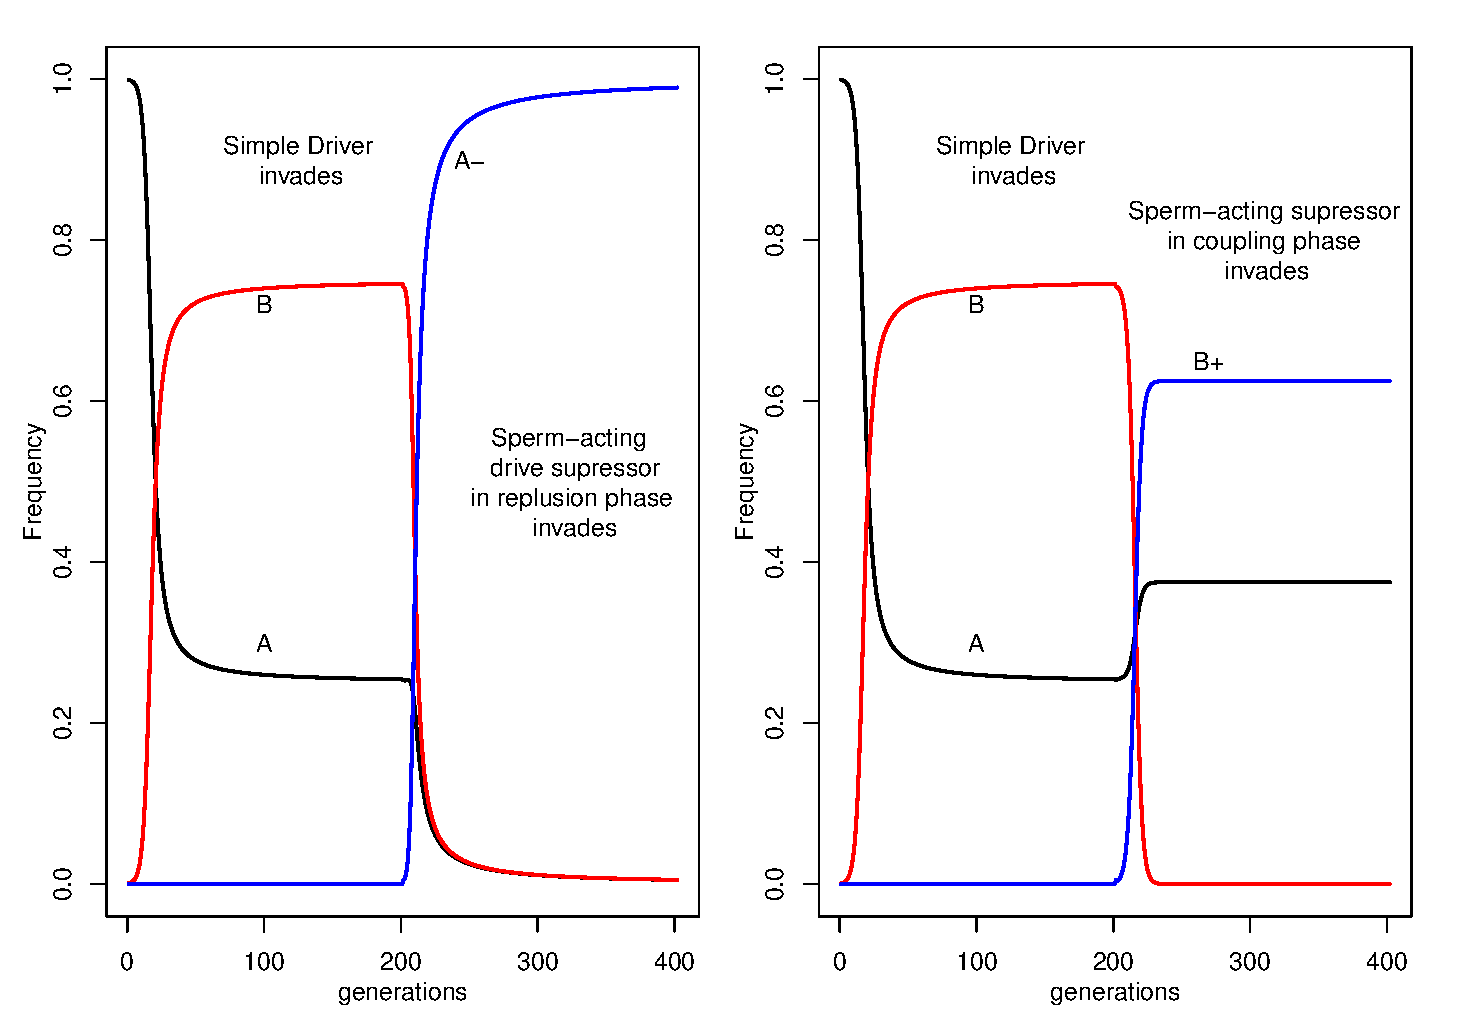
\includegraphics[width = 0.8 \textwidth]{Figures/trajectories_of_sperm_based_supressors.eps} 
% \caption{Trajectories of two sperm-based supressors of drive. Possibly
% merge this figure the 3 allele cartoon}  \label{Trajectories_of_supressors}
% \end{figure}



%%%%%%%%%%%%%%%%%%%%%%%%%
% TWO LOCUS MODEL [modify (general) / facilitate (helps ) / prevent (stops)] 
%%%%%%%%%%%%%%%%%%%%%%%%%

Above, we explored a model of an allele drove in females when signaled by a complementary allele in sperm.  
We complement this single locus model %of an allele with pleiotropic effects in both sexes, 
	with  an alternative model of two linked loci - one a female driver, 
	and the other a sperm allele which modifies the effect of drive upon fertilization. 
In this model, a female meiotic driver with no sperm-dependency 
	initially reaches drive-viability equilibrium (with two alleles
	$A$ and $B$ are the ancestral non-driver and driver alleles). 
Subsequently, a sperm-acting modifier of female meiotic drive arises tightly
        linked to this balanced locus (effectively creating a third
        allele/haplotype at this locus). Tight linkage offers the best
        chance for a collaboration to evolve between a driver and
       an enhancer of the drive, as recombination breaks up drive haplotypes \citep{Thomson1974,Charlesworth1978,Haig1991}. 
In addition tight linkage between female driver and sperm modifier is consistent with the nature of well characterized drive systems which are often maintained as polymorphic inversions with numerous linked modifiers (CITE).

%\yb{??In the SUPP we explore the dynamics of a sperm modifier of female drive unlinked to the female driver??} 

%%%sperm-acting facilitator
We first consider a sperm-acting enhancer of
	female meiotic drive tightly linked to the $B$ background, 
	generating a third `$B^{+}$' allele (i.e. the non-recombining haplotype of a
        driver allele and sperm-acting drive modifier). 
This new allele acts in sperm to increase the effectiveness of both
	the $B$ and  $B^{+}$ drive in $AB$ and $AB^{+}$ heterozygotes (see Figure \ref{Eggsperm_3_allele_cartoon})
%	for a simple schematic of this drive model.  
Naively, the $B^{+}$ may spread by capitalizing on the additional drive it causes; however,  
	this is not the case for a few simple reasons. 
First, the sperm-acting drive facilitator (the novel $B^{+}$ haplotype) 
	arises when the ancestral driver ($B$) is at drive-selection balance, 
	and therefore immediately suffers a homozygous fitness cost.  
Worse yet, a novel $B^{+}$ haplotype most often helps 
	the $B$  allele drive ($B^+$ sperm meeting $AB$ eggs), because $B$ is initially more common than $B^{+}$. 
As $B^{+}$ facilitates $B$ these interactions frequently form 
	$BB^{+}$ heterozygotes that suffer the same fitness costs as $BB$. 
Therefore, sperm-acting drive facilitator alleles experience a profound disadvantage 
	in this scenario, even more so than under the previous two allele model. 
We have found no parameter range of this
	three allele system that allows the sperm-acting drive facilitator $B^{+}$ to
	invade the population. 

%%%sperm-acting drive suppressors
While  sperm enhancement of a female drive cannot displace a polymorphic female driver, sperm based drive suppression can. 
%	that is sperm-acting alleles that act to restore  fairness of female meiosis, can. %If these sperm-acting drive suppressors arise on
If a sperm-acting allele that restores fairness to female meiosis arises on
	the non-driving $A$ background (creating a third allele $A^{-}$), 
	or is unlinked to the drive locus, it readily invades a population segregating
	for the drive system ($AB$, see Figure and Equations \ref{A-} and \ref{unlinked}).  
This allele lowers the frequency of the original drive system (perhaps to zero),
	and spreads to fixation if it does not carry strong fitness costs
	(Figure \ref{Eggsperm_3_allele_cartoon} and \ref{Trajectories_of_supressors}A). 
This result is consistent with previous work showing that drive suppressors unlinked to, or in repulsion phase with drivers usually invade polymorphic drive systems \citep[e.g. ][]{Brandvain2012}.  

More surprisingly, sperm-acting suppressors of female drive can spread
	even when tightly linked to the original drive system (Figures \ref{Eggsperm_3_allele_cartoon} and \ref{Trajectories_of_supressors}B). 
The $B^{-}$ haplotype (representing the tightly linked drive/drive suppressor complex) displaces the original driver 
	by driving when not costly, but avoiding low fitness homozygotes by disrupting drive when transmitted to sperm. %  ($BB^-$ and $B^-B^-$). 
Despite displacing the ancestral driver (the $B$ haplotype), the equilibrium frequency of the $B^-$ haplotype is often lower than that of $B$ \yb{(point to supp?)}. 

%\gc{Do we mention the In and Om locus here or in the discussion as a
%	 potential e.g. Do we mention the fact that the frequency of these
%	 newly invade sperm dodging alleles can be lower than the original system?}\\

\section*{Discussion}

Sexual reproduction is a high-stakes event that determines what gets transmitted to the next generation.  
As a consequence of this intense competition, alleles that gain a transmission advantage during reproduction 
	can succeed evolutionarily, even if they lower the 
        fitness of the population, 
	the mother whose offspring they will inhabit, 
	or the organism in which they reside. 
This generates numerous conflicts  \cite{Burt2006} including sexual conflicts between mates \cite{Arnqvist2005}, 
	and conflicts between alleles that are over-transmitted in meiosis and the organisms they injure while doing so. 
Such conflicts and their resolution likely play a major role in the structure and evolution of many basic biological processes \citep{Rice2013}.

It seems that allowing sperm to influence the outcome of female meiosis would generate a confluence of these potential conflicts -- 
	sperm could actually assist an allele that distorts female meiosis.
However, this is not the case.
We find that an allele which acts through sperm to distort female meiosis in its favor %YB [too awkward / unclear?] 
	can rarely spread through a population if it bears any cost. 
Additionally, when this self-promoting driver can spread, it can only rarely 
	be maintained as a protected polymorphism, and due to its positive frequency dependence 
	it spends very little time at intermediate frequency.
As such, this type of exploitation cannot generate a sustained genetic conflict.
It is therefore unlikely
	that female oogenesis and meiosis will evolve to prevent their effect.  
This likely explains why females can delay the completion of meiosis until after fertilization 
	without risking exploitation by collaborations by female
        drivers and sperm alleles.
%Male modification of recombination rates. \yb{trying to think through this \dots{}}

Why is it that an allele that biases female meiosis in its favor can generate a genetic conflict, but an allele in sperm that assists this female driver cannot? 
So long as the transmission advantage of female meiotic drive outweigh the organismal fitness cost to heterozygotes the female driver can spread when rare, and it increases in 		
	frequency until the fitness cost experienced when homozygous balances the transmission advantage.
By contrast a sperm promotor of female drive is only effective when matched with a heterozygote female -- meaning that when rare this allele rarely enhances female drive. 
Even worse, when it does so it will preferentially find itself in a low fitness drive homozygote. 
Not only are drive-promoting sperm alleles unable to create a sustained genetic conflict, 
	but alleles in sperm with the opposite effect - that is those that prevent their own drive through female meiosis do maintain a polymorphisms and 
	provide evolution  with time and opportunity to further minimize drive.
This is because such drive suppressing alleles reduced their chances
of forming low fitness homozygotes. 
In fact, an allele in sperm which causes the alternate allele to drive can be favored (FIG), a counterintuitive result 
	consistent with the tenuous evidence that the non-driving
        $ln^-$ allele is over transmitted through female meiosis in $ln^-/ln^+$ heterozygote when fertilized by $ln^+$
        sperm \cite{agulnick, Pomiankowski1993}.   
More generally, alleles that act through sperm to
 reduce the opportunity of female meiotic drive regardless of linkage or phase. 


%More generally both linked and unlinked alleles may often spread that act through sperm to
%reduce the opportunity of female meiotic drive in order to disable
%segregating drive systems, by for example reducing the mechanistic
%asymmetries that female drivers exploit. 





The interests of fertilizing sperm and female are quite well aligned during syngamy -- producing a viable and potentially fit offspring. 
%As noted above there are even opportunities for coevolution between sperm-based suppressors of female meiotic drive and the female genome.
Thus it seems plausible that aspects of oogenesis may actively evolve to facilitate the influence of sperm on ensuring a fair  outcome of female meiosis which generates fit offspring.
In light of that it is interesting to consider whether the phylogenetic variation in the stage of oogenesis when fertilization takes place reflects not
	only species' different reproductive ecologies, but also different selection pressures shaping the interaction of sperm alleles with female meioses. 
%\gc{Add short paragraph about sex chromosomes here? XY systems don't care. ZW systems (males ZZ, females ZW). If there is
%sex ratio distortion how could this play out?}


%\yb{DOES THIS GO ANYWHERE? }

% Males can potentially influence the outcome of meiosis even before fertilization. 
% For example in Drosophila and other taxa, sperm accessory
%         gland proteins (ACPs) increase the female recombination rate
%         \cite{SOMEthING}, and there is some evidence that there is
%         variance across male genotypes in there effect on female
%         recombination rate \cite{Stevison2012}.
% Presumably this is a pleiotropic consequence of the resolution of double strand breaks initiated by the stressful/toxic composition of ACPs. 
% However, a pleiotropic effect of this is to increase the recombination rate which can decrease the effectiveness of female meiotic drivers
% active during MI \citep{Brandvain}. 
% We speculate that other effects of sperm on female meiosis may also be tolerated by females as a way of ensuring meiotic fairness -- 
% 	that is females evolve to allow male influence on female meiosis in cases in which the male influence is  egalitarian. 

%Gametogenesis and meiosis are common times for genetic conflict. 
%This is a consequence of the fact that as the set of alleles that consitute
%	an individual are in the process of parting ways, 
%	with only a subset of them being assured transmission.
%In constrast, the perspective of the fertilizing sperm's genome is different, it has to live with the consequences of any distortion it causes 
%to female meiosis through the entire next life cycle of the organism. 
%It is therefore in the interest of the fertilizing sperm's genome to
%make a high fitness zygote even if that means alleles in sperm
%disrupting other copies of themselves from gaining a 
%transmission advantage through female meiosis.
  \appendix


\section*{Appendix}
Our appendix highlights some of our derivations and analytical results from: 
	the standard female meiotic drive (Model 1); a sperm
	dependent female meiotic drive (Model 2); a male genotype dependent
female meiotic drive (Model 3); and more complex two locus sperm
dependent drive (Models 4-6). %changed this to minimize confusion with refs, figs, equations, etc.

%Below, we highlight some of our derivations and analytical results. 
%The fitness of genotype, $g$ is $w_g$ independent of its sex, and its 
All models include a biallelic locus with non-driving and driving alleles in frequencies $f_A$ and $f_B$, 
	respectively, while more complex models include more loci and/or alleles.  
Transmission rules describing the outcomes of all matings in each
	models are presented in a \yb{Supplementary Worksheet}. 
The fitness of genotype, $g$ is sex-independent and equals $1$, $1-h_s$, and $1-s$ for genotypes $AA$, $AB$, and $BB$, respectively. %  and  $w_{AA} = 1$, $w_{AB} = 1-s_h$, and $w_{BB}=1-s$. 
Genotypic frequencies  equal  $f_g$ for adults in the current generation, 
	$f_g'$ in the next generation of zygotes (i.e. after recombination, random mating, drive, and syngamy, but before selection)
	and $f_g''$ in adults after selection. 
After a complete generation $f_g'' = f_g' w_g/\bar{w}$, where $\bar{w}$ is the population mean fitness and equals $\Sigma w_g f_g'$. 
%All models include a biallelic locus with non-driving and driving alleles in frequencies $f_A$ and $f_B$, respectively, while more complex models include more loci and/or alleles.  
%Transmission rules describing the outcomes of all matings in each
%models are presented in a \yb{Supplementary Worksheet}, and complete derivations of our analytical approximations are in the
%\gc{Mathematical Supplement}.  
Because many of our analyses assume Hardy Weinberg Equilibrium (HWE), we note which analytical results are approximations. 
We verify these approximations with exact numerical iterations in Supplementary Figures and Supplementary Scripts, and detail the derivation of these approximations in our Mathematical Supplement. 



\subsection*{Models 1-3. Single-locus drive}
\subsubsection*{Model 1. Traditional driver}
In the standard female drive model, meiosis in males is fair such that $A/B$ heterozygotes contribute $A$ and $B$ alleles with equal probabilities; however, $A/B$ females transmit the $B$ allele with probability $d>1/2$. 
After drive and random mating, genotype frequencies are 
	$f_{AA}'=f_A (f_{AA }+ f_{AB} (1 - d))$, 
	$f_{AB}'=f_A (f_{BB} + f_{ABd}) + f_B (f_{AA} + f_{AB} (1 - d))$,
	and $f_{BB}= f_B (f_{AB} d + f_{BB})$. 
%Assuming fitnesses $w_{AA}=1$, $w_{AB}-1 s_h$ and $w_{BB}=1-s$, 
%Frequencies of genotype, $i$, after drive and selection are 
%	\begin{equation} f_i''= f_i'w_i/\bar{w}\end{equation}
%	where $w_i$ is genotypic fitness, and mean fitness, $\bar{w} = \Sigma f_i'w_i$. 
As detailed above, exact frequencies after drive, random mating and selection are $f_g''= f_g'w_g/\bar{w}$. 
Assuming HWE, a rare driver will spread when $s_h
        \lessapprox(2d-1)/(1+2d)$, and will fix when $s\lessapprox d -1/2 +
        3 s_h /2- d s_h$. This later inequality reduces to
        $s\lessapprox(2d-1)/2$ when the cost of drive is fully
        recessive. \gc{isn't this last expression exact?}
	
\subsubsection*{Model 2. Single locus, sperm-dependent drive.}
Our single-locus model of sperm dependent drive resembles the traditional driver with the caveat that the $B$ allele drives in heterozygous females only when fertilized by $B$ bearing sperm. 
Therefore, genotype frequencies after drive are 
	$f_{AA}'=f_A^2$, 
	$f_{AB}'=f_A f_B+f_B (f_{AA} + f_{AB}(1 - d)) $,
	and $f_{BB}'= f_B (f_{AB} d + f_{BB} )$. 
%As above, exact frequencies after drive, random mating and selection are $f_i''= f_i'w_i/\bar{w}$. 
We iterate exact genotype frequency recursions ($f_g''= f_g'w_g/\bar{w}$) over generations to produce the frequency trajectories shown in the inset
Figure \ref{Invasion_space} by plotting \gc{$f_B=f_{BB}+ \frac{1}{2}f_{AB}$}
over time. %, and to assess the analytical approximations, below.
 \gc{To assess invasion or fixation criteria, \yb{as well as bistability points,} we iterate this system and
testing whether $f_B$ increases over a grid of parameters. }

% the $B$ allele In our first scenerio allele $A$ is the ancestral allele and allele
%$B$ is our sperm dependent drive allele.
%The sperm dependence of the drive is a form of assortative
%transmission (mating), and so we have to keep track of the genotype frequencies.
%Our genotype frequencies at birth are $x_{AA},~x_{AB},$ and
%$x_{BB}$. These three genotypes have fitnesses $w_{AA},~w_{AB},$ and
%$w_{BB}$, which are identical between males and females. Because 
%fitnesses are equivalent in both sexes, genotypic frequencies
%are identical in males and females, but in the following
%equations they are marked with $\Mars$ and $\Venus$ respectively to
%allow the reader to more easily follow the logic. 
%The frequency of the three genotypes at birth in the next generation is:
%\begin{equation}
%x'_{BB} =\frac{1}{\bar{w} } \Big( w_{BB} x_{BB}^{\Venus} (w_{BB} x_{BB}^{\Mars} +\frac{1}{2}
%  w_{AB} x_{AB}^{\Mars} ) + w_{AB} x_{AB}^{\Venus} (d w_{BB}
%  x_{BB}^{\Mars} +\frac{1}{2} d
%w_{AB} x_{AB}^{\Mars} ) \Big),  \label{eqn.A1}
%\end{equation}
%\begin{equation}
%x'_{AA} =\frac{1}{\bar{w} } \Big(  w_{AA} x_{AA}^{\Venus} (w_{AA} x_{AA}^{\Mars} + \frac{1}{2}
%   w_{AB} x_{AB}^{\Mars}) + w_{AB} x_{AB}^{\Venus}(\frac{1}{2} w_{AA} x_{AA}^{\Mars}+ \frac{1}{2} 
%  w_{AB} x_{AB}^{\Mars}) \Big),  \label{eqn.A2}
%\end{equation}
%and
%\begin{eqnarray}
%x'_{AB} = & \frac{1}{\bar{w} } \Big( w_{AA} x_{AA}^{\Venus}  ( w_{BB}  x_{BB}^{\Mars} + \frac{1}{2}
%  w_{AB}  x_{AB}^{\Mars} ) +w_{BB} x_{BB}^{\Venus} ( w_{AA}  x_{AA}^{\Mars} + \frac{1}{2}
%  w_{AB}  x_{AB}^{\Mars} )  \nonumber \\
%& + x_{AB}^{\Venus}(\frac{1}{2}  w_{AA}  x_{AA}^{\Mars}+\frac{1}{2} (1-d)
% w_{AB}  x_{AB}^{\Mars} + \frac{1}{4}  w_{AB}
 %x_{AB}^{\Mars} + (1-d)  w_{BB}  x_{BB}^{\Mars} ) \Big) \label{eqn.A3}
%\end{eqnarray}
%where the mean fitness of the population is
%\begin{equation}
%\bar{w} = w_{AA} x_{AA}+w_{AB}  x_{AB} +w_{BB}  x_{BB}.
%\end{equation}
%We can then iterate this recursion over generations, for
%example to produce the frequency trajectories shown in the inset
%Figure \ref{Invasion_space} by plotting $x_{BB}+ \frac{1}{2}x_{AB}$
%over time. We can also use this to assess the
%invasion criteria for the allele by starting allele B at very low
%frequency, and seeing if it increases across the generations.

\paragraph{Recessive fitness cost of self-promoting driver:} %When the self-promoting driver has a recessive fitness cost, $s$ genotype frequencies after selection and drive equal
%\begin{equation}	x'_{BB} =\frac{x_{B}^2(1-s)}{\bar{w} }  \Big( F+(1-F)(x_{B}+2x_{A} d) \Big) 	\end{equation}
%\begin{equation}	x'_{AA} =\frac{1}{\bar{w} }  \Big(x_{A}^2\Big) 	\end{equation}
%and
%\begin{equation}	x'_{AB} =\frac{2 x_{A}x_{B} }{\bar{w} }  \Big(1-x_{B}(d-1/2)(1-F) \Big)	%\end{equation}
When fully recessive, the change in frequency of the self-promoting driver across generations equals 
\begin{equation}
\Delta f_B=f_A f_B^2 \left( [1-F][ d(1-2 f_A s) - f_B s-1/2] - s  F \right)/\bar{w}
\label{deltadriver}
\end{equation}
where $F$ is the deviation from genotypic frequencies expected under Hardy-Weinberg. % Trying to clarify some.   \gc{Hardy Weinberg Expectations} (HWE). 
%For analytical solutions presented above, we assume that $F$ equals zero. 
Assuming HWE  ($F=0$) a common, recessive, self-promoting driver invades if $s\lessapprox(2 d - 1)/(4 d)$, and fixes if
 $s\lessapprox(2d-1)/2$. 
 Therefore, when 
\begin{equation}
(2 d - 1)/(4 d)  \lessapprox  s  \lessapprox  (2d-1)/2\label{ineqA}
\end{equation} 
a recessive, self-promoting driver will deterministically fix if drift,
 	mutation, or migration pressure bring its frequency above
\begin{equation} 
f^*_{B\text{ recessive}} \approx (1-2d+4ds)/(2s(2d-1)) \label{bistab_homozy_approx}
\end{equation}
 but it will be lost if it is introduced below this frequency. 
 %(i.e. this is an unstable equilibrium point). 
% In Supplementary Figure \ref{Bistab_homozyg_cost_fig} we show
% this approximation condition for bistability andd how it compared to
% that obtained using the recursion. 
Compared to exact results (Supplementary Figure \ref{Bistab_homozyg_cost_fig}), Equations
 \gc{\eqref{ineqA} and} \eqref{bistab_homozy_approx} offer reasonable, but imperfect approximations. 
%s_h and seems to serve as a lower bound to the true unstable equilibrium frequency. 

\paragraph{Cost of driver in heterozygotes:} %We explored a more complex model where the self-promoting driver has a cost, $s_h$ in heterozygotes (so $w_{AB} = 1-s_h$) in addition to the cost $s$, in homozygotes.
When the fitness of drive heterozygotes is compromised ($s_h>0$), a self promoting driver cannot invade when rare.
This results from the fact that
when rare %($f_B \ll 1$) 
$B$-bearing sperm rarely
encounter heterozygous eggs ($\sim f_B^2$) but the allele still pays a
cost in heterozygous individuals ($\sim f_B$). 
%Model construction is similar to that above.
%So long as there is any heterozygous fitness cost (i.e. $s_h > 0$) the self-promoting driver cannot invade when rare;
However, this system too, is bistable -- as the driver becomes more frequency it is more often fertilized by a driving sperm and therefore drives more effectively.
%Assuming no deviation from Hardy-Weinberg a self-promoting driver with a heterozygous fitness cost 
This allele deterministically fixes if its frequency exceeds some threshold, $f_B^*$.
Assuming HWE, this threshold equals 
\begin{equation}
	f_B^* \approx \frac{a_1+\sqrt{a_1^2+8 s_h a_2}}{2 a_2}
	\label{thresh2}
\end{equation}
where, $a_1=1-2 ds_h+4 d s-2 d-3 s_h$ and $a_2=2(s-s_h)(2d-1)$.
Comparison of Equation \ref{thresh2} to exact results obtained by a
simple parameter search (Supplementary Figure \ref{bistable_additive})
show that this approximation is reasonably correct for small
parameter values; \yb{however, this approximation underestimates $f_B^*$ for large parameter values, presumably because they result in strong departures from HWE.}
 %range of other costs to the drive alleles other than a
%simple recessive cost, for example an additive cost. We modified the recursions given in eqn
%\ref{eqn.A1}-\ref{eqn.A3} to feature an additive cost $s$ for each
%copy of the $B$ allele. A none recessive cost to the drive allele can
%cause bistability of the drive allele. The B allele is unable to enter
%the population when rare, this results from the fact that
%when the allele is rare ($x_B \ll 1$) sperm carrying it rarely
%encounter heterozygous eggs ($\sim x^2$) but the allele still pays a
%cost in heterozygous individuals.  By contrast, when the B allele is common ($x_B
%\gg 0$) encounters between heterozygous eggs and $B$ allele sperm
%become more common allowing drive to occur this can allow the $B$
%allele to spread when common. In Supplementary Figure
%\ref{bistable_additive} we show the unstable equilibrium frequency
%above which the $B$ allele can invade. This equilibrium frequency was found by a simple
%parameter search.  \gc{wonder if a bit of work could find this}

\subsubsection*{Model 3. Single locus, paternal genotype dependent drive:}
We now turn to the case when female meiotic drive depends on paternal genotype.
%\paragraph{Dominance} we also explored a model where
%the genotype of the male who produced the fertilizing sperm affects female drive,
%instead of just the allelic type of the sperm.
 We assume a heterozygous female will transmit the $B$ allele 
  with probabilities  $\frac{1}{2}$,  $d_{het}\geq 1/2 $ or $d_{hom}\geq d_{het}$, 
%YB RE-PARAMETERIZING  %  $\frac{1}{2}$,  $\frac{1}{2} + h(d-\frac{1}{2}) $ or $d$,  YB RE-PARAMETERIZING 
 when mated with to $AA$, $AB$, or $BB$ males,  respectively. 
  In this model, genotype frequencies after drive, mating and selection are 
  	$f_{AA}'' =   w_{AA}\left( f_{AA} [2 f_A + f_{AB} ] + f_{AB}^2 [1 - d_{het}] \right)/(2\bar{w})$,
	$f_{AB}'' =   w_{AB}(f_{AA} [f_B + f_{AB}/2] + f_{AB} f_B + f_{BB} [ f_A - f_{AB} d_{hom}])/\bar{w}$, 
	and 	$f_{AB}'' =   w_{AB}(f_{AB} (f_{AB} d_{het}/2 + f_{BB} d_{hom}) + f_{BB} f_B)/\bar{w}$. 
% Above, $d > 1/2$ and $h$ ($0 \geq h \geq 1$) acts to specify the dominance of the $B$
%allele's effect on female meiotic drive through the males genotype.
%YB TRY_1 We assume that in a mating between a heterozygous female and an $AA$, $AB$, or $BB$ male, the female will transmit the $B$ allele 
% with probabilities  $\frac{1}{2}$,  $\frac{1}{2} + h(d-\frac{1}{2}) $, and $d$, respectively.
  %Here $d > 1/2$ and $h$ ($0 \geq h \geq 1$) acts to specify the dominance of the $B$
%allele's effect on female meiotic drive through the males genotype.
% GC ORIGINAL  We assume that if a
%heterozygous egg ($AB$) is fertilized by a sperm with the following
%male ($\Mars$) genotypes the $B$ allele will be transmitted through
%female meiosis with the following probabilities \\
%\begin{tabular}{cccc}
%$\Mars$ geno. & AA & AB  & BB\\
%P(B). & $\frac{1}{2}$ &  $\frac{1}{2} + h(d-\frac{1}{2}) $ & $d$ 
%\end{tabular}\\
%where $d > 1/2$ and $h$ ($0 \geq h \geq 1$) acts to specify the dominance of the $B$
%allele's effect on female meiotic drive through the males genotype. 
%We set up a set of recursions using a recessive sex independent cost to
%the driver, similar to those in eqn.
%\ref{eqn.A1}-\ref{eqn.A1}, but now featuring these male genotype
%transmission probabilities. 

If the cost of drive is fully recessive (i.e. $s_h=0$), assuming HWE, 
	a rare paternal genotype dependent driver invades when 
	$s\lessapprox (d_{het}-1/2)/(d_{het})$, and a common paternal genotype dependent driver fixes when 
	$s\lessapprox d_{hom}-1/2$, approximations well supported by exact results (Supplementary Figure \ref{Effect_of_dominance}).
Specifically, when drive in heterozygotes is large relative to that in homozygotes, 
	\begin{equation} d_{het}  \gtrapprox 1/(3-2d_{hom}) \label{polymale} \end{equation}
	fixation criteria are more stringent than invasion criteria, 
	and therefore some values of $s$ can maintain a stable polymorphism. 
Under these parameter values, a rare paternal genotype dependent driver 
	can increase in frequency as drivers gain a transmission advantage and suffer 
	no fitness cost when heterozygous eggs are fertilized by 
	$A$-bearing sperm of heterozygous males. 
As the frequency of the $B$ allele increases, 
	occur more often as a homozygote, and so will be unable to 
	avoid producing unfit homozygote zygotes, leaving it trapped in
	the population at frequency $f_{B\text{ pat}}^*$. 
Assuming HWE, a recessive fitness cost ($h_s=0$), and dominance of driver ($d_{het}=d_{hom}$) this equilibrium frequency is
\begin{equation}f_{B\text{ pat}}^*\approx2 (1 + 2d_{hom}[s - 1])/([2 s - 1][2d_{hom}- 1]) \label{eqmale} \end{equation}
By contrast, when $d_{het} \lessapprox 1/(3-2d_{hom})$ the case is reversed, and the model is bistable.
%In Supplementary Figure \ref{Effect_of_dominance} we show the invasion
%criteria for both the A and B alleles when they are rare. 
%We find a narrow parameter range where B 
%can invade but not fix.{eqmale}
%This corresponds to B being less than fully recessive (i.e. $h>0$) and to a modest cost in homozygotes. 
%This combination of parameters reflects the fact that when the allele is rare, 
%it can increase in frequency due to fertilization of heterozygous eggs
%by sperm from heterozygote males, where the sperm do not themselves
%carry the allele. But as the B allele becomes common it will frequently be
%present in the homozygous state in males, and so will be unable to
%avoid the production of unfit homozygote zygotes leaving it trapped in
%the population. 


\subsection*{Models 4-6. Two-locus, sperm-dependent drive.} 
Assuming that a traditional driver segregates at its equilibrium frequency (Model 1), we investigate the evolution of tightly linked (Models 4 and 5), and unlinked sperm-dependent modifiers of drive. 
In models 4 and 5, we treat this two loci system as if it consists of
three alleles: $A$, $B$ and $C$, corresponding to the case \gc{when the
sperm-modifier arises once, tightly linked to one or other of the
alleles (such that recombination is unexpected). }
In all cases, fitness is independent of the drive modifier, so, $w_{AA}=1$, $w_{AB}=1-s_h$, and $w_{BB} = 1-s$. 
We assume the traditional driver is transmitted to $d_0$ of gametes from female heterozygotes  when fertilized by wild-type sperm, and $d_1=d_0+\epsilon$ when fertilized by a sperm acting drive modifier.

\subsubsection*{Model 4. Drive-modifier in coupling phase:}
When the $C$ allele is tightly linked to the driver allele, 
	genotypic fitnesses equal $w_{AC}=w_{AB}=1-s_h$, and $w_{BC}=w_{CC}=w_{BB}=1-s$. 
Assuming HWE, a recessive fitness cost to drive, and assuming that the $A/B$ locus is at its equilibrium frequency, the change in frequency of a rare drive modifier is
\begin{equation}
	\Delta C\approx -\epsilon f_C \frac{ 1-2 d_0 (-2 d_0+s+2)+\sqrt{2} \sqrt{s (2 d_0 (d_0(s-2)+2)-1)}}{2 \bar{w}(1-2 d_0)^2}
\end{equation}
%YB Considered this ugly math more impressive.
For all parameters sustaining a polymorphism at the drive locus ($s>d_0-1/2$), this corresponds to a decrease in frequency of the $C$ allele when it enhances drive ($\epsilon >0$ -- the $B^+$ model, above), 
	and a decrease in frequency of the $C$ allele when it suppresses drive ($\epsilon <0$ -- the $B^-$ model, above). 
More generally even when the cost of drive is not fully recessive, the $B^-$ allele will invade and fix under all parameters sustaining a previous polymorphism at the drive locus (see Mathematical Supplement). 
%When the C allele acts to suppress drive for all parameters sustaining a polymorphism at the drive locus ($s>d_0-1/2$)
%We address two questions concerning the $C$ allele - can it invade when rare  and can it fix when common?
%Although our analytical approximations (see our \gc{Mathematical supplement}) do not reveal simple inequalities like those above,
%	graphical exploration of analytical results show that this mutant is lost when it enhances drive ($\epsilon>0$ - the $B^+$ allele, above),
%	and spreads from rarity to fixation when it suppresses drive ($\epsilon<0$ - the $B^-$ allele, above).	
%This result is supported by exact numerical iterations, as well
%\yb{FIG?}. \gc{Lets not bother}

\subsubsection*{Model 5. Drive-modifier in repulsion phase:}
When the $C$ allele is tightly linked to the non-driver, 
	genotypic fitnesses equal $w_{CC}=w_{AC}=w_{AA}=1$, and $w_{BC}=1-s_h$. 
Assuming HWE, a recessive fitness cost to drive, and assuming that the $A/B$ locus is at its equilibrium frequency, the change in frequency of a rare drive modifier is
\begin{equation}
	\Delta C \approx -\epsilon f_{C^-}^2 \frac{ \left(2 d_0 s-\sqrt{2} \sqrt{s (2 d_0 (d_0 (s-2)+2)-1)}\right)}{2\bar{w}s (2 d_0 -1) }. \label{A-}
\end{equation}
For all values of interest ($0<s<1$, $0.5<d_0<1$), the change in frequency a rare $C$ is positive when it decreases drive (i.e. $\epsilon <0$, corresponding to the $A^-$ model, above), a result which hold qualitatively for a common $C$ allele, as well (Mathematical Supplement). 
%We address two questions concerning the $C$ allele - can it invade when rare  and can it fix when common?
%Again, while simple inequalities are lacking, 
%	graphical exploration of our analytical results, and exact numerical iteration \yb{FIG?} shows that this modifier only spreads from rarity to fixation when it suppresses drive ($\epsilon<0$ - the $A^-$ allele, above). 
Somewhat counterintuitively, the spread of the $A^-$ allele is substantially slower than that of the $B^-$ allele (it is on the order of $C^{2}$ rather than $C$). 
This is because the $A^-$ allele will never occur in drive-homozygotes and therefore only spreads by preventing itself from the cheating of the driver.

\subsubsection*{Model 6. Unlinked drive-modifier:}
%\gc{Can we use something other than F, as that was HWE deviation}
For the unlinked, model we introduce another locus where drive is modified in A/B females fertilized by $M$ allele, 
	while the wild-type $L$ does not influence drive. 
Assuming HWE and linkage equilibrium, the change in frequency of a rare unlinked, sperm-acting drive modifier is 
\begin{equation} \Delta M =-\epsilon f_A f_B (f_B s + s_h (fA - fB) ) \frac{f_M}{\bar{w}}  \label{unlinked} \end{equation}
% an $F$ allele increases in frequency when 
%	$-\epsilon f_A f_B (f_B s + s_h (fA - fB) ) >0$, corresponding to any level of drive suppression ($\epsilon<0$) 
Thus, a rare drive suppressor ($\epsilon<0$) will spread so long as  the fitness cost of the driver does not display over- or under-dominance. 
Notably, this result holds while assuming complete linkage equilibrium, and therefore sperm suppression of female meiotic drive is likely more powerful than female enforced systems which usually spread due to the indirect benefit of avoiding drive haplotypes \citep[e.g. ][]{Brandvain2012}.  
The spread of this driver does not, however, depend on assumption of HWE, and linkage equilibrium - exact results resemble analytical approximations. 
%\paragraph{three allele system}
%$x_{AA}$, $x_{AB}$,$x_{AB'}$, $w_{BB'} x_{BB'}$, $w_{B'B'} x_{BB}$, $w_{B'B'} x_{B'B'}$
%We denote the frequency of the three genotypes in the population at birth are
%$x_{AA}$, $x_{AB}$, $x_{AB'}$, $x_{BB'}$, $x_{BB}$, $x_{B'B'}$. 
%The mean relative fitness of the population is 
%\begin{equation}
%x_{AA}+x_{AB}+ x_{AB'}+ w_{BB'} +x_{BB'}+w_{B'B'}x_{BB} + w_{B'B'} x_{B'B'} 
%\end{equation}
%The frequency of the genotypes in meiotic-cells of female adults is 
%\begin{equation}
%\frac{1}{\bar{w}}\Big( x_{AA}, ~x_{AB},~ x_{AB'},~ w_{BB'} x_{BB'},~ w_{B'B'}x_{BB},
%~w_{B'B'} x_{B'B'} \Big)
%\end{equation}
%The frequency of fertilization events can be found by combining these
%female frequencies with the frequency of the three alleles in sperm is
%\begin{eqnarray}
%x_A = & x_{AA} + \frac{1}{2} x_{AB}+ \frac{1}{2} x_{AB'} \\
%x_B = & w_{BB}  x_{BB} +   w_{BB'} \frac{1}{2} x_{BB'}+ \frac{1}{2} x_{AB} \\
%x_{B'} = & w_{B'B'}  x_{B'B'} +   w_{BB'} \frac{1}{2} + x_{BB'}+ \frac{1}{2} x_{AB'}  
%\end{eqnarray}
%in combination with the transmission probabilities given in Figure
%\ref{Eggsperm_3_allele_cartoon}A.

% \gc{Alternatively we could give the table below:}

% \begin{table}
% \begin{tabular}{lllll}
% \hline 
%   &  \multicolumn{4}{c}{Sperm genotype}   \\
%   &  & A & B & B'  \\
% $\Venus$ geno. & Freq.  & $x_{AA} + \frac{1}{2} x_{AB}+ \frac{1}{2} x_{AB'} $ & $ w_{BB}  x_{BB} +   w_{BB'} \frac{1}{2} x_{BB'}+
% \frac{1}{2} x_{AB}$ & $ w_{B'B'}  x_{B'B'} +   w_{BB'} \frac{1}{2}
% x_{BB'}+ \frac{1}{2} x_{AB'}  $\\
% \hline\\
% AA & $x_{AA}$ &  & & \\
% AB & $x_{AB}$ &  & & \\
% AB' & $x_{AB'}$ &  & & \\
% BB' & $w_{BB'} x_{BB'}$ &  & & \\
% BB & $w_{B'B'} x_{BB}$ &  & & \\
% B'B' & $w_{B'B'} x_{B'B'}$ &  & & \\
% \end{tabular}
% \caption{ALTERNATIVELY I COULD FILL IN THIS MATRIX  with genotype }
% \end{table}
\bibliography{refs}

\section*{Supplementary Material}


\begin{figure}

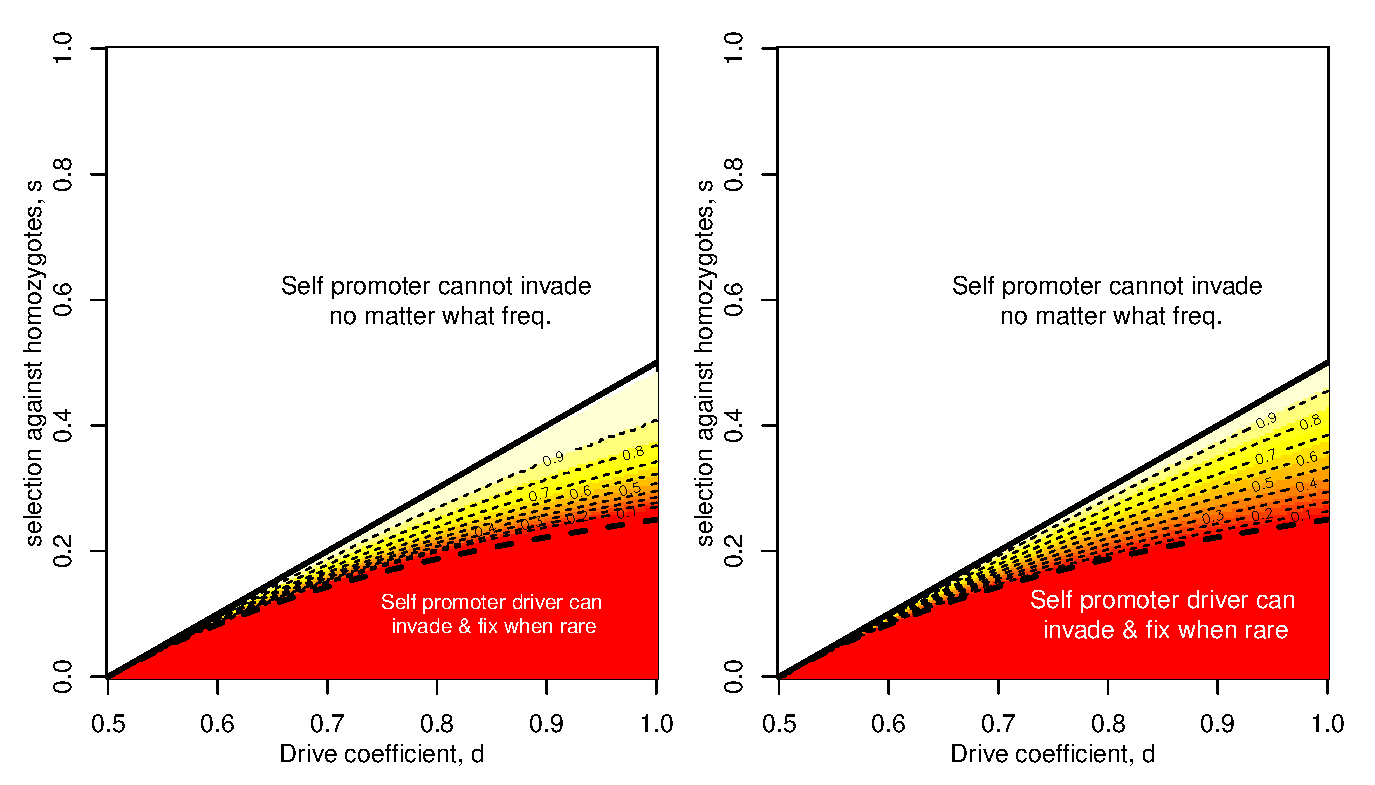
\includegraphics[width = 0.5
          \textwidth]{../Scripts/homozyg_bistability.eps}
\caption{Invasion analysis for a self-promoting female meiotic drive allele with
  recessive costs (selection coefficient $s$), showing the region of
  bistability. The colors, and the thin dashed contours, indicate the
  frequency the allele must be above to invade the population (note
  that these alleles reach fixation conditional on invading). In the
  white area the allele can not invade ($x \geq1$), in the solid red
  area the allele can invade and fix when rare. In the left panel we
  show the results obtained by a grid search using the recursion, on
  the right we show the approximation obtained assuming that HWE
  holds. }  
\label{Bistab_homozyg_cost_fig}
\end{figure}

\begin{figure}
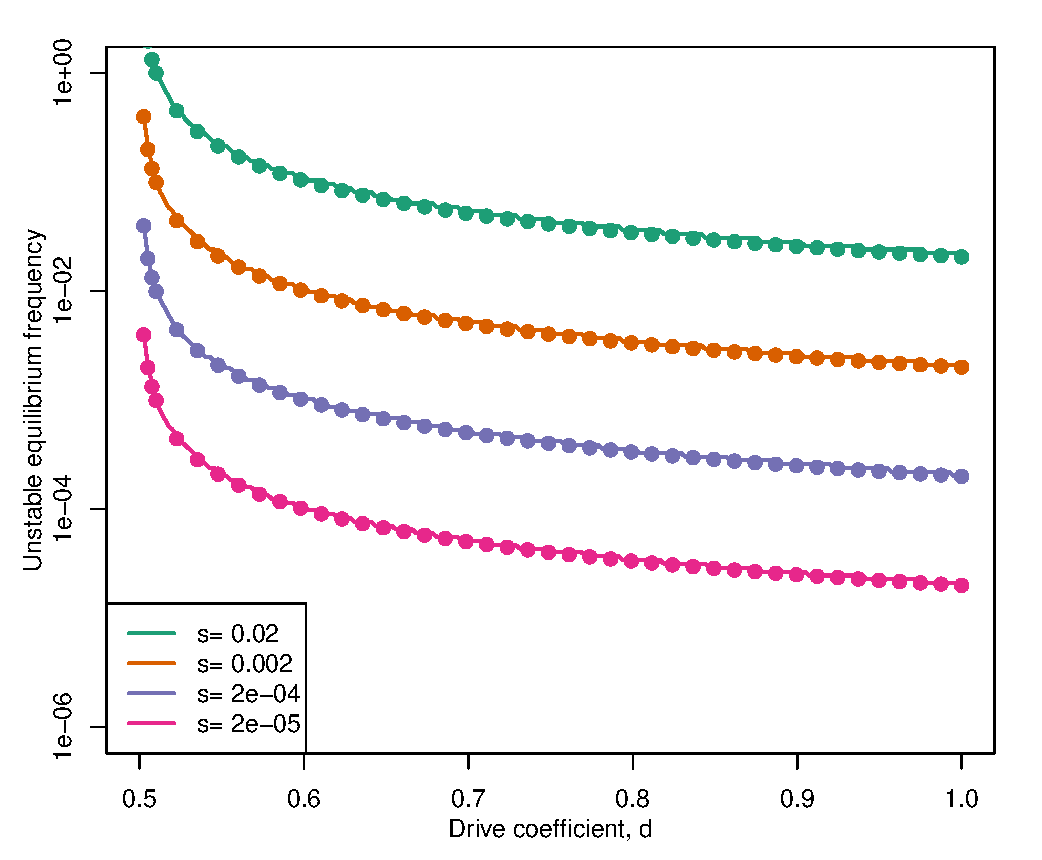
\includegraphics[width = 0.8 \textwidth]{Figures/bistable_x_vs_d_additive_s.eps} 
\caption{The unstable equilibrium frequency for a self-promoting
  female meiotic drive allele with an additive cost ($s_h=s/2$) as a
  function of the drive parameter. The solid line shows results
  obtained using the recursion, the dots our approximation given by \eqref{thresh2}/}  \label{bistable_additive}
\end{figure}

\begin{figure}
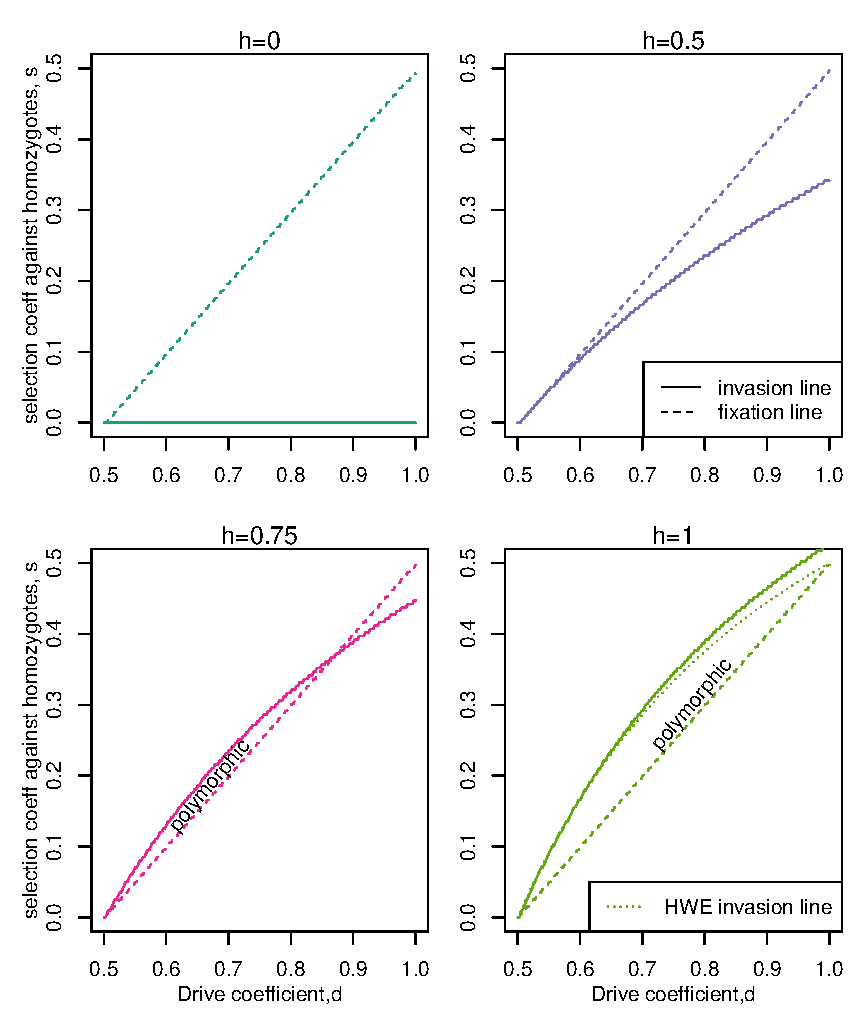
\includegraphics[width = 0.8 \textwidth]{../Scripts/effect_of_dominance_on_invasion_space_four_graph.eps} 
\caption{Invasion analysis of an allele whose effect
 on female meoisis is mediated by the genotype of the fertilizing
 male.  As above wee assume a heterozygous female will transmit the $B$ allele 
  with probabilities  $\frac{1}{2}$,  $\frac{1}{2} + h(d-\frac{1}{2}) $ or $d$, 
 if she mated with a n $AA$, $AB$, or $BB$ male,  respectively.  The allele suffers a recessive fitness cost $s$.  
 The four panels correspond to different dominance relationships.
In the parameter space below the invasion (solid) line the self-promotor
 driver can invade. In the parameter space below the fixation (long
 dash) line the self-promotor can fix in the population. In the last
 two panels the invasion line is above the fixation line and so the
 allele can be maintained as a polymorphism in that thin slice of
 parameter space between the two lines. These results were 
  obtained using the recursion. In the final panel we show the
  fixation line (small dashes) as predicted by our HWE approximation
  ($(d_{het}-1/2)/d_{het}$), see the `dominance' section of the
  Appendix for more details.
}  \label{Effect_of_dominance}
\end{figure}

\end{document}




